\chapter{Aplikacja mobilna}

\section{Projekt i implementacja oparte na wzorcu MVP (Dorota Tomczak)}
\par Pracę nad aplikacją mobilną rozpoczęto od stworzenia bazowego projektu składającego się z kilku pustych widoków, do których to następnie można było dodawać kolejne funkcjonalności. W celu zachowania najlepszych praktyk programistycznych zdecydowano się na oparciu projektu o wzorzec architektoniczny MVP (ang. model-view-presenter). Jest to wzorzec szczególnie nadający się do implementacji w aplikacjach mobilnych na systemy Android ze względu na aktywności (ang. activity), które pełnią funkcję środkowej warstwy – widoku (ang. view). W implementacji wzorca w tym projekcie widok jest pasywny (ang. passive view) tzn. widok powinien odpowiadać jedynie za wyświetlanie interfejsu i użycie bibliotek związanych z Androidem. Cała logika aplikacji ma być zawarta w prezenterze (ang. presenter), który pełni funkcję kontrolera.

\par Zastosowanie wzorca MVP pozwoliło na zachowanie porządku w strukturze projektu i przejrzysty podział na warstwy. Do każdej aktywności, czyli nowego ekranu w aplikacji, utworzono interfejs zwany kontraktem (ang. contract) zawierający opis interakcji jakie mogą zajść pomiędzy prezenterem a widokiem, a w szczególnych przypadkach również między prezenterem a adapterem, który odpowiada za wyświetlanie listy obiektów (rys.~\ref{fig:launcherContract}). Klasy aktywności i prezentera implementują interfejsy zawarte w kontrakcie, prezenter jest wstrzykiwany do widoku, a referencja widoku jest przekazywana do prezentera w konstruktorze.

\begin{figure}[h]
\centering
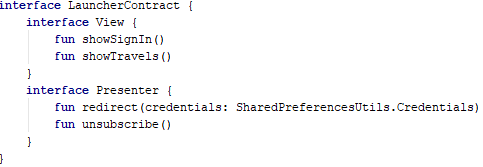
\includegraphics[width=\linewidth]{launcherContract}
\caption{Prosty kontrakt widoku odpowiadający za przekierowanie do widoku logowania lub listy podróży.}
\label{fig:launcherContract}
\end{figure}
\FloatBarrier

\par Do wstrzykiwania zależności, w tym prezenterów do aktywności, wykorzystano popularny framework \textit{Dagger 2} \cite{Dagger 2}, co ostatecznie okazało się być nie najlepszym wyborem – należało dodać dwie dodatkowe klasy do każdej aktywności, co przy dużej ich liczbie wygenerowało wiele plików o bardzo podobnej strukturze. Ponadto niemalże jedynymi wstrzykiwanymi obiektami były obiekty klas prezenterów. 

\section{Komunikacja z aplikacją serwerową (Anna Malizjusz)}
\par Aplikacja mobilna musi komunikować się z RESTowym API udostępnianym przez serwer. W tym celu wykorzystano klienta o nazwie Retrofit 2 \cite{Retrofit library}. Dzięki niemu w łatwy sposób można zaimplementować interfejs odpowiedzialny za wysyłanie zapytań i odbieranie odpowiedzi.

\par Napisano kilka klas, aby umożliwić prostą komunikację w aplikacji. Interfejs \textit{ServerApi} (rys.~\ref{fig:serverApi}) zawierał zbiór metod z odpowiednimi adnotacjami @PUT, @POST, @GET, @DELETE i nazwami punktów końcowych. Metody nie wymagały implementacji przez programistów, ponieważ ich obsługa należała do odpowiedzialności klienta Retrofit 2.

\begin{figure}[h]
\centering
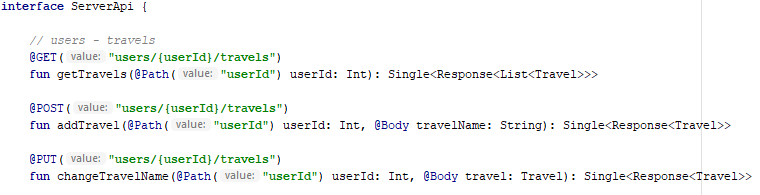
\includegraphics[width=\linewidth]{serverApi}
\caption{Przykładowa zawartość interfejsu używanego przez Retrofit 2.}
\label{fig:serverApi}
\end{figure}
\FloatBarrier

\par Dodatkowo zaimplementowano klasę pomocniczą konfigurującą klienta. Udostępniała ona zmienną (ang. property), która była przygotowanym interfejsem do komunikacji. Ustawiono w niej adres serwera REST, a także konwertery przeprowadzające serializację obiektów do formatu JSON oraz deserializację z otrzymanego ciągu znaków w formacie JSON do obiektu będącego instancją danej klasy. Skorzystano z klasy \textit{GsonConverter}, która jest oferowana przez Retrofit API. Wykorzystano wzorzec projektowy interceptor implementując klasę \textit{AuthTokenInterceptor}, którego rolą było dodanie do każdego zapytania nagłówka (ang. header) z lokalnie zapisanym tokenem identyfikującym użytkownika. Interceptor aplikacji jest wywoływany zawsze i tylko jeden raz, nie wpływają na to przekierowania ani ponawianie zapytań. Aby zintegrować interfejs używanego klienta z interceptorem, należało dodać dodatkowego klienta -- \textit{OkHttpClient} \cite{OkHttpClient}. Pochodzi z biblioteki OkHTTP, którą również można było wykorzystać do komunikacji aplikacji mobilnej z serwerem, jednak postawiono wybrać Retrofit 2 z uwagi na mniejszy poziom skomplikowania oferowanego API.

\par Rezultatem każdego zapytania jest struktura \textit{Single<Response<T> >}, gdzie T jest oczekiwanym typem zwracanego obiektu. Obiekt \textit{Single} informuje o tym, że jest spodziewana pojedyncza odpowiedź. \textit{Response} jest strukturą zdefiniowaną w projekcie inżynierskim. Zawiera kod odpowiedzi opisywany szerzej przy sposobie implementacji błędów, a także także pole \textit{data} z przesłanymi przez serwer danymi.


\section{Logika rejestracji i logowania (Anna Malizjusz)}
\par Rejestracja użytkownika polega na podaniu trzech informacji: adresu email oraz dwukrotnym podaniu hasła. Każde z tych pól jest walidowane. Adres e-mail powinien mieć formę \\xxx@yyy.zzz, gdzie xxx, yyy i zzz są dowolnymi ciągami znaków. Hasło nie powinno być trywialne. Musi zawierać co najmniej jedną cyfrę, jedną wielką i jedną małą literę, a także mieć przynajmniej 8 znaków długości. Poprawność walidacji została sprawdzona testami jednostkowymi (rys.~\ref{fig:registerUnitTestResult}).

\begin{figure}[h]
\centering
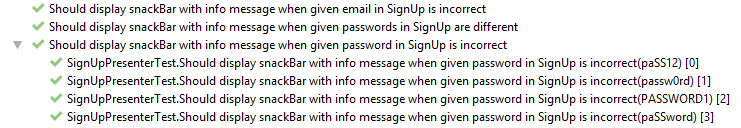
\includegraphics[width=\linewidth]{registerUnitTestResult}
\caption{Testy jednostkowe sprawdzające poprawność sposobu walidacji formularza rejestracji}
\label{fig:registerUnitTestResult}
\end{figure}
\FloatBarrier


\section{Wyszukiwanie atrakcji turystycznych i zakwaterowania (Anna Malizjusz)}
\par Dodanie konkretnego miejsca do planu dnia jest możliwe po jego wyszukaniu. W tym celu stworzono ekran umożliwiający wybranie obiektu z mapy. Na wyświetlanym obszarze są widoczne pinezki odpowiadające obiektom w podanej okolicy.

\par Głównym komponentem widoku wyszukiwania jest \textit{SearchView} \cite{SearchView}. Dzięki temu na ekranie widać pole, w które można wpisać nazwę lub początek nazwy miasta i wybrać je z listy. Mapa automatycznie przeniesie się do wskazanego miejsca. Implementacja mechanizmu podpowiedzi znajduje się w klasie \textit{CitySuggestionProvider}, dziedziczącej po \textit{ContentProvider} \cite{ContentProvider}. Kluczowym było nadpisanie metody \textit{query(Uri, String[], Bundle, CancellationSignal)}, która zwracała wynik do widoku. Używając interfejsu komunikacji z serwerem aplikacja pobierała listę proponowanych miast, a \textit{CitySuggestionProvider} zwracał je w formie kursorów.

\par Po wybraniu pinezki jednego z wyświetlanych obiektów na ekranie pojawia się nazwa miejsca, a także możliwość pokazania jego szczegółów. Zostało to osiągnięte dzięki użytemu układowi o nazwie \textit{SlidingUpPanelLayout} \cite{SlidingUpPanelLayout}. Pozwala on na rozwinięcie i późniejsze ukrycie widocznego na dole obszaru ze szczegółowymi informacjami. Te same dane są w późniejszym etapie dostępne po wybraniu elementu z planu dnia. Z tego powodu postanowiono wyodrębnić układ pól z informacjami, zdefiniować go w osobnym pliku i wykorzystać go zarówno w widoku wyszukiwania, jak i widoku detali obiektu.

\par Uwzględniono szczególny przypadek, jakim jest wyszukanie zakwaterowania. Jeżeli aplikacja wykryje, że dany obiekt jest miejscem noclegu, zaproponuje dodatkowo dodanie daty wykwaterowania. Końcowym efektem będzie pojawienie się dwóch elementów w planach dni. Pierwszy z nich jest podpisany jako zakwaterowanie (ang. check in), a drugi jako wykwaterowanie (ang. check out). Wystawienie oceny jest możliwe tylko dla elementu reprezentującego drugie z tych wydarzeń.


\section{Tworzenie planów podróży (Dorota Tomczak)}
\par Tworzenie planów podróży jest kluczową funkcją aplikacji. Stworzenie takiego planu jest możliwe, gdy użytkownik ma przypisaną do swojego konta dowolną podróż. Dodawanie do niej kolejnego elementu planu zostało zrealizowane poprzez prosty formularz, który zawiera:
\begin{itemize}
\item rozwijaną listę z kategoriami miejsc odpowiadającą wybranym kategoriom z \textit{Here API} \cite{Here},
\item pole z nazwą miejsca, które po dotknięciu przekierowuje do ekranu wyszukiwania, a po wybraniu obiektu wypełnia się automatycznie,
\item pola od dnia i od godziny, po których dotknięciu otwierają się dialogi odpowiednio z kalendarzem i zegarem,
\item pola analogiczne do dwóch powyższych, jeśli wybrano kategorię Zakwaterowanie, oznaczające dzień i godzinę wykwaterowania,
\item pole z adresem, które wypełnia się automatycznie po wyszukaniu obiektu,
\item pole na notatki, które są potem możliwe do edycji.
\end{itemize}

\par Po zatwierdzeniu formularza zostaje on poddany walidacji – wszystkie pola oprócz notatek muszą być wypełnione, a dla kategorii \textit{Zakwaterowanie} (ang. \textit{Accommodation}) czas zakwaterowania nie może być przed czasem wykwaterowania. Jeśli formularz pomyślnie przejdzie próbę walidacji, nowy element planu podróży zostaje utworzony.
Elementy planu dnia wyświetlają się w formie chronologicznej listy rozdzielonej separatorami z datami. Do implementacji tego rozwiązania posłużył adapter, który na podstawie typu elementu określa jaki układ xml (ang. layout xml) wyświetlić – czy ten dla elementu planu czy daty. Aby oba typy mogły być używane przez adapter, muszą dziedziczyć po wspólnym interfejsie, którym jest \textit{DayPlanItem} z jedną metodą, która zwraca typ obiektu.
\par Jednak zanim nowy element planu dnia może zostać przekazany do adaptera i wyświetlony na ekranie jest najpierw dodawany do kolekcji typu \textit{TreeSet}, która sortuje znajdujące się w niej elementy po wyniku zwracanym przez metodę \textit{compareTo(other: PlanElement): Int}, zaimplementowaną w klasie dodawanych elementów. Następnie tworzona jest lista składająca się z separatorów oraz wspomnianych elementów – po sprawdzeniu pola \textit{fromDate} elementu następuje decyzja, czy rozdzielić elementy nowym separatorem z dniem czy nie. Tak przygotowana lista trafia do adaptera i efektem jest widok posortowanych chronologicznie elementów planów dni w podróży.


\section{Implementacja skanowania dokumentów z użyciem OpenCV (Dorota Tomczak)}
\par Aplikacja umożliwia zrobienie zdjęcia, wybranie czworokątnego obszaru oraz takie przycięcie i modyfikację kolorów fotografii, aby uzyskać efekt skanu. W początkowych założeniach zakładano skorzystanie z gotowej biblioteki, która poza wymienionymi wyżej funkcjonalnościami dokonywałaby automatycznej detekcji krawędzi, jednak ze względu na brak darmowych i dostosowanych do potrzeb rozwiązań zdecydowano zaimplementować skaner od podstaw bazując na projekcie open-source \textit{SimpleDocumentScanner-Android} \cite{SimpleDocumentScanner-Android}.

\par Wykonanie fotografii jest możliwe jeśli użytkownik nadał aplikacji odpowiednie uprawnienia. Są one weryfikowane przy każdej próbie dodania skanu. Jeśli aplikacja została do tego uprawniona, tworzony jest plik tymczasowy w pamięci urządzenia, a następnie otwierany jest widok kamery za pomocą intencji (ang. intent) utworzonej poprzez podanie do konstruktora nazwy odpowiedniej akcji. Zdjęcie wykonane przez użytkownika jest zapisywane w utworzonym wcześniej pliku tymczasowym a jego ścieżka przekazywana do aktywności (ang. activity) skanera, aby umożliwić w niej jego wyświetlenie i modyfikację.

\par W celu zaimplementowania możliwości wyboru obszaru zdjęcia poprzez gesty użytkownika dodano specjalną klasę dziedziczącą po \textit{ImageView} \cite{ImageView}. Taka klasa mogła zostać następnie dodana do układu xml skanera, a zaimplementowane w niej metody pozwoliły na rysowanie i przeciąganie czterech linii złączonych końcami i tworzących czworokąt. Końce czworokąta są reprezentowane przez cztery zmienne typu \textit{PointF} zawierające informacje o ich położeniu na ekranie urządzenia. Po każdym wykryciu gestu przeciągnięcia linii łączącej punkty, obliczane jest ich nowe położenie, a następnie ponownie złączane są linią (rys.~\ref{fig:scan1}). Gdy użytkownik zatwierdzi zaznaczony obszar punkty transformowane są z ich współrzędnych na urządzeniu na współrzędne na zdjęciu.

\par Kolejnym etapem jest uzyskanie efektu zeskanowanego dokumentu (rys.~\ref{fig:scan2}). Aby móc to osiągnąć zastosowano bibliotekę \textit{OpenCV} \cite{OpenCV}, której pliki źródłowe musiały zostać dołączone do projektu aplikacji w postaci modułu. Aby ograniczyć rozmiar aplikacji wynikowej, który znacznie wzrósł po dodaniu biblioteki, usunięto jej klasy, które nie były potrzebne do realizacji funkcjonalności. Najważniejszymi operacjami, które dostarczyła OpenCV jest transformacja perspektywiczna (ang. perspective transform), która w ogólności zajmuje się przekształceniem trójwymiarowego świata do dwuwymiarowego obrazka, oraz progowanie obrazu (ang. thresholding), czyli metoda segmentacji obrazu pozwalająca uzyskać obraz binarny z obrazu kolorowego. Otrzymany skan po zastosowaniu tych dwóch operacji i innych pomocniczych może być przez użytkownika zachowany lub odrzucony. W tym pierwszym przypadku zostaje on przesłany na serwer.

\begin{figure}[h]

\centering
\subfloat[Zaznaczanie obszaru do skanowania.\label{fig:scan1}]{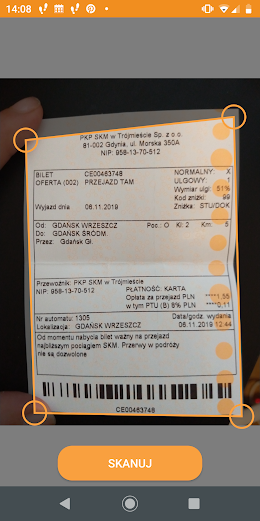
\includegraphics[width=0.4\textwidth]{scan1}}
\hfill
\subfloat[Skan wynikowy po transformacjach zdjęcia.\label{fig:scan2}]{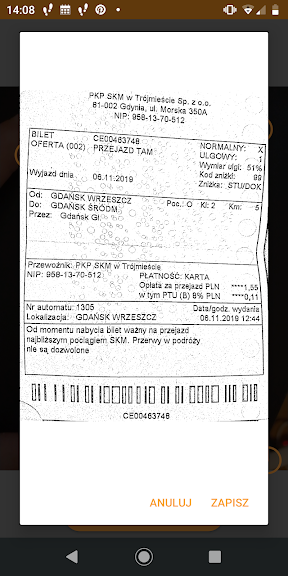
\includegraphics[width=0.4\textwidth]{scan2}}
\hfill

\caption{Skanowane biletu.}
\label{fig:Eimage1}
\end{figure}
\FloatBarrier

\section{Obsługa przesyłania i pobierania plików (Dorota Tomczak)}
\par Aby umożliwić użytkownikom korzystanie ze swoich kont na różnych urządzeniach oraz udostępnianie stworzonych przez siebie podróży, wynikła konieczność przesyłania dodanych zdjęć na serwer, zamiast przechowywania ich lokalnie na urządzeniach mobilnych. Zdjęciami w aplikacji mogą być wykonane skany lub fotografie dodane do poszczególnych podróży, a ich przesyłanie odbywa się przy pomocy RESTowego API udostępnianego przez serwer, jak zostało to opisane w podrozdziale 5.2. Zapytania za to odpowiadające są dodatkowo opatrzone adnotacją \textit{@Multipart}, aby umożliwić przesyłanie całych plików w ciele (ang. body) żądania, natomiast pliki przekształcane są na obiekt typu \textit{MultiPartBody.Part}. Gdy plik zostanie odebrany po stronie serwera następuje próba jego zapisu w ustawionym w konfiguracji folderze przez \textit{FileStorageService}, czyli serwis do przechowywania plików. Następnie ścieżka do pliku jest dodawana do bazy wraz z innymi niezbędnymi informacjami umożliwiającymi jego identyfikację.

\par Ładowanie plików w aplikacji zostało zrealizowane dzięki bibliotece \textit{Glide} \cite{Glide}, która pozwala na zwiększenie efektywności tego procesu poprzez automatyczne korzystanie z pamięci podręcznej urządzenia i optymalizację rozmiaru zdjęcia. Znając adres, pod którym znajduje się plik, użycie wspomnianej biblioteki jest bardzo proste, dlatego na większą uwagę zasługuje proces wysyłania fotografii przez serwer. Plik o wskazanej nazwie zostaje załadowany jako obiekt typu \textit{Resource} przez \textit{FileStorageService}, a następnie konstruowana jest odpowiedź serwera, która w ciele zawiera otrzymany zasób. Odpowiedź jest dodatkowo opatrzona nagłówkiem \textit{Content-Disposition}, który zawiera informację o tym, że plik ma zostać potraktowany jako załącznik. 

\section{Dodawanie użytkowników do znajomych oraz wyświetlanie listy znajomych (Karolina Makuch)}

\par W celu umożliwienia użytkownikowi udostępniania planu podróży znajomym dodano do aplikacji funkcjonalność odpowiadającą za wyszukiwanie konkretnych użytkowników. Została ona zrealizowana poprzez  wykorzystanie komponentu \textit{SearchView} \cite{SearchView} zawierającego pole umożliwiające wpisanie ciągu znaków. Podczas wprowadzania kolejnych liter zostają wyświetlane podpowiedzi w czasie rzeczywistym. Aktualizują się  przy każdej zmianie wyrazu. Uwzględniają one wszystkie adresy mailowe zarejestrowanych w aplikacji użytkowników zaczynających się od podanego ciągu znaków.

\par W tym celu została stworzona klasa implementująca abstrakcyjną klasę \textit{ContentProvider} \cite{ContentProvider}. Po wysłaniu odpowiedniego zapytania zostaje utworzony \textit{MatrixCursor} \cite{MatrixCursor} zawierający dwie kolumny: identyfikator użytkownika oraz jego adres mailowy. Po otrzymaniu odpowiedzi od serwera dla każdego użytkownika zostaje utworzony wiersz, który następnie jest dodawany do kursora. Wyświetlana jest tylko kolumna zawierająca adres mailowy.

\par Kursor został również wykorzystany w celu umożliwienia dodania wybranego użytkownika do znajomych. Podczas kliknięcia na wybrany wiersz zostaje wywoływana nadpisana metoda \textit{onSuggestionClick} obiektu klasy \textit{SearchManager} \cite{SearchManager}. Pobiera ona potrzebne dane wybranej pozycji z tablicy \textit{MatrixCursor’a} \cite{MatrixCursor}.

\par Do eliminacji przypadkowych działań zostało wykorzystane okno dialogowe wymagające potwierdzenia  zamiaru dodania wybranego użytkownika do znajomych. W tym celu została wykorzystana klasa \textit{AlertDialog} \cite{AlertDialog}. Po wyrażeniu zgody  oraz w przypadku poprawnego wykonania metody użytkownik otrzymuje powiadomienie stworzone poprzez wywołanie konstruktora klasy \textit{Snackbar} \cite{Snackbar}.

\par W tym samym oknie pod polem do wyszukiwania znajduje się lista znajomych użytkownika. Została ona dodana jako liniowa warstwa (\textit{LinearLayout} \cite{LinearLayout}) umożliwiająca odświeżanie widoku poprzez szybkie przesunięcie palcem po ekranie (\textit{SwipeRefreshLayout} \cite{SwipeRefreshLayout}). Implementuje ona tryb usuwania.

\par Powiązanie dwóch użytkowników poprzez oznaczenie ich jako znajomych zostało zrealizowane poprzez dołączenie do bazy danych osobnej tabeli (app user friend)  przechowującej potrzebne informacje (identyfikator użytkownika oraz identyfikator znajomego). Dodawanie jest jednostronne. Znajomy danego użytkownika nie jest zobowiązany do posiadania go na swojej liście znajomych.

\par Po stronie serwera zostały dodane pliki umożliwiające komunikację z wspomnianą powyżej tabelą oraz wykonywaniu potrzebnych zapytań. Zostały zaimplementowane wszystkie bazowe, niezbędne do komunikacji z bazą danych zapytania. Oprócz nich przygotowano również zapytanie zwracające wszystkie adresy mailowe nieznajomych użytkowników zawierających wpisany ciąg znaków.

\section{Udostępnianie podróży znajomym (Karolina Makuch)}

\par  Udostępnianie podróży jest możliwe po dodaniu użytkownika do listy znajomych. W momencie wybrania ikony udostępnienia pojawia się okno dialogowe (\textit{DialogFragment} \cite{DialogFragment}) zawierające znajomych użytkownika w formie listy wyboru (ang. checkbox) nie mających dostępu do danego planu podróży. Implementacja zapytania do bazy danych została pokazana na rysunku poniżej (rys.~\ref{fig:getFriendsBySharedTravel}). Podczas implementacji została nadpisana metoda \textit{setMultiChoiceItems} w celu umożliwienia udostępnienia planu wielu znajomym podczas jednej czynności.
\par  Po wybraniu osób, zatwierdzeniu decyzji oraz poprawnym wykonaniu metody użytkownik otrzymuje powiadomienie stworzone poprzez wywołanie konstruktora klasy \textit{Snackbar} \cite{Snackbar}. Odpowiednie powiadomienie zostaje również wyświetlone w sytuacji niewybrania ani jednego znajomego oraz potwierdzeniu wykonania czynności.
\par  Każdy użytkownik mający dostęp do podróży posiada prawa do edycji jej planu. Podczas wykonywania czynności udostępniania wybranemu znajomemu zostaje przypisana dana podróż poprzez dodanie powiązania w odpowiedniej tabeli.

\begin{figure}[h]
\centering
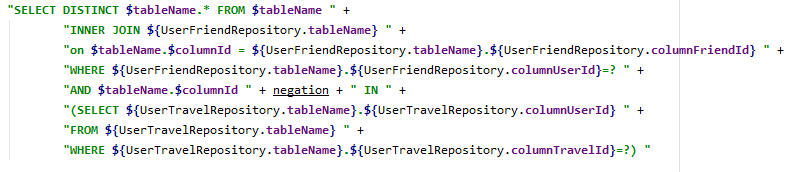
\includegraphics[width=\linewidth]{getFriendsBySharedTravel}
\caption{Zapytanie zwracające listę adresów mailowych znajomych danego użytkownika nieposiadających dostępu do wybranej podróży.}
\label{fig:getFriendsBySharedTravel}
\end{figure}
\FloatBarrier

\section{Udostępnianie planu dnia w medium społecznościowym (Karolina Makuch)}
\par  Po dłuższym przytrzymaniu poszczególnego elementu planu pojawia się \textit{dymek}  (\textit{PopupMenu} \cite{PopupMenu}) zawierający trzy czynności do wyboru. Jedną z nich jest możliwość udostępnienia wybranego punktu w medium społecznościowym. Postanowiono wybrać jedno z najpopularniejszych –- \textit{Facebooka} \cite{Facebook}. W tym celu wykorzystano akcję wysyłającą (\textit{ACTION.SEND}) za pomocą intencji (\textit{Intent} \cite{Intent}).
\par  W przypadku znalezienia aplikacji Facebook na telefonie użytkownika, zostanie on automatycznie przekierowany do publikowania posta na własnej \textit{tablicy}. Domyślną treścią jest link do map HERE \cite{mobileHere} z wyszukanym miejscem z elementu planu dnia. W celu pobrania właściwego odnośnika  zostało zaimplementowane odczytywanie wartości parametru widoku (ang. view) znajdującego się w odpowiedzi w formacie JSON (z wykorzystaniem \textit{JsonParser} \cite{JsonParser}). Odsyłacz do wyników zapytania został pobrany z bazy danych. Wykonanie analizy (ang. parse) wyniku zapytania wymagało utworzenia osobnego wątku.
Wykonanie tej operacji na głównym wątku zablokowałoby interfejs użytkownika. 
\par Początkowo planowano inną domyślną treść. Miała ona zawierać najważniejsze informacje na temat wybranego elementu planu. Niestety zarówno wbudowany w Androidzie moduł  udostępniania, a także \textit{API Facebooka} nie udostępnia tej możliwości. Problem ten został zgłoszony ponad 7 lat temu, lecz nie został rozwiązany \cite{FacebookBug}. Pola \textit{"EXTRA SUBJECT"} oraz \textit{"EXTRA TEXT"} są pomijane w momencie próby udostępniania domyślnej zawartości w aplikacji Facebook. Z racji możliwości załączania zdjęć, linków oraz plików multimedialnych (np. wideo) rozważane było zamienienie tekstu na plik obrazu oraz dodanie go do akcji. Brane również pod uwagę było przeniesienie domyślnej wiadomości do schowka oraz wyświetlenie komunikatu informującego użytkownika z prośbą o wklejenie wiadomości.
\par Jednakże stwierdzono, że takich akcji nie powinno się wymagać od użytkownika. Ostatecznie postanowiono, że najlepszym rozwiązaniem będzie zdecydowanie się na wspomniany wcześniej odsyłacz do wyszukanego miejsca z mapy HERE \cite{mobileHere}. Dzięki czemu treść posta zostanie utworzona przez użytkownika umożliwiając mu zachowanie własnego charakteru pisania.

\section{Manualna realizacja planu (Karolina Makuch)}
\par  Kolejną akcją dostępną w \textit{dymku} pojawiającym się po przytrzymaniu poszczególnego elementu jest manualna realizacja planu dnia. Początkowa treść akcji dla nowo powstałego nieukończonego jeszcze elementu planu dnia brzmi \textit{Oznacz jako ukończony} (ang. \textit{Mark as completed}). W przypadku oznaczenia części składowej planu jako zrealizowany tekst automatycznie zmienia się na \textit{Oznacz jako nieukończony} (ang. \textit{Mark as incompleted}) oraz zwiększa się stopień przeźroczystości odpowiedniego elementu listy. Postanowiono oznaczać zrealizowane plany poprzez wygaszenie kolorów elementów danego planu zmniejszając wartość kanału \textit{alfa} (ang. alpha).
 \par Zdecydowano się umożliwić użytkownikowi cofnięcie wprowadzonych zmian w przypadku wykonania niechcianego kliknięcia, świadomie rezygnując z wymagającego potwierdzenia okna dialogowego. Stwierdzono duże prawdopodobieństwo wykonywania tej akcji w pośpiechu. Dodatkowe kliknięcie wydłużyłoby czas wykonywania akcji oraz mogłoby to irytować użytkownika.
\par  Oznaczenie planu jako wykonany zostało umożliwione dzięki dodaniu odpowiedniej kolumny do tabeli zawierającej plany dni. Dzięki temu każdy użytkownik mający dostęp do podróży ma możliwość wykonania tej czynności i jej efekty są widoczne dla wszystkich uczestników wyprawy.

\section{Tryb usuwania (Magdalena Solecka)}
\par Usuwanie podróży, skanów, elementów planu dnia oraz znajomych jest możliwe przez wybranie z menu kontekstowego, pojawiającego się po przytrzymaniu obiektu, opcji usuń. Powoduje to przejście do trybu usuwania zaimplementowanego z użyciem trybu akcji (ang. Contextual Action Mode) \cite{contextualActionMode} oferowanego przez Android. Na żądanie usunięcia wybranych elementów wysłane do serwera, odpowiada on listą identyfikatorów poprawnie usuniętych  obiektów, które następnie są usuwane z widoku aplikacji. Dzięki temu nie jest konieczne wysyłanie dodatkowego żądania w celu zaktualizowania listy po stronie klienta.
\par Funkcje, które należy zaimplementować w celu poprawnego działania trybu usuwania zostały wyodrębnione do osobnych interfejsów zamkniętych w Kontrakcie DeleteContract. Uwspólniono również klasę DeleteActionModeToolbar odpowiadającą za inicjalizację i zniszczenie trybu usuwania. Ułatwiło to pracę nad funkcjonalnością usuwania obiektów dodanych na późniejszym etapie prac.
